% =============================================================================


\chapter{Introduction}
In~the~software industry, the~great, accessible and~testable code is crucial
for~modern business, and~the~best way for~us to~test and~share it is
through APIs\footnote{API is an~abbreviation for~an~Application Programming
Interface which is a~set of~protocols and~tools for building application
software.}. They are supposed to~connect engineers, allow for~the~sharing
of~developments, let companies add value to~the~products and~create an~ecosystem
of~shared knowledge. To~fulfill these tasks they have to~be clear, accessible
and~most importantly human and~machine readable. However, despite their
importance there hasn't been an~industry standard for documentating nor~testing
them.

This thesis aim to~solve the~problem of~documentating and~testing the~APIs.
The~goal is to~design and~develop an~application having an~innovative user
interface with~regard to~clarity and~simple use, aimed to~developers, even
in~case of~large interfaces. The~application will be based on~Swagger
framework that provides a~way to~automate API generation.
The~application will provide not~only API reference, but mainly
the~functionality to~create extensive test cases from~the~listed web services.

% TODO
% DP - Pridat do designu vetu o - based on~live mockups.. and~later
%      on~PatternFly Framework.

The~thesis is organizes as~follows. Chapter~\ref{Preliminaries} gives
definitions needed to~follow the~thesis and~explains web services
and~RESTful APIs in~detail. Chapter~\ref{Technologies} focuses on~technologies
that are going to~be used for~implementation of~the~application. Chapter~\ref{Design}
describes the~application design, wireframes and~mockups.
The~last Chapter contains an~overall summary of~the~designed solution and~final
thoughts on~the~work done within the~thesis.


% =============================================================================


\chapter{Preliminaries and Definitions}
\label{Preliminaries}
This chapter will gradually introduce terms necessary to~follow the~thesis.
In~the~first sections, we will go over the~basic terminology and~establish
notion of~remote interfaces and~web services. In~the~next section, we will
provide an~explanation what APIs are, and~why it is important to~automate their
testing. The~last section covers the~introduction of~a~Swagger framework \cite{Swagger} 
and~its importance to~the~thesis.

\section{Understanding the Web Services}
\label{WebServices}
A~web service is a~software system designed to~support interoperable machine
to~machine interaction over a~network. It is a~collection of~open protocols
and~standards used for exchanging data between applications or~systems. Software
applications written in~various programming languages and~running on~various
platforms can use web services to~exchange data over the~computer networks like
the~Internet in~a~manner similar to~interprocess communication on~a~single
computer.

In~the~past, web services used mostly SOAP\footnote{Simple Object Access
Protocol is a~protocol specification for~exchanging structured information
in~the~implementation of~web services in~the~computer networks.} over HTTP
protocol, allowing less costly interactions over the~Internet. In~a~2004,
the~W3C extended the~definition of~web services about \uv{REST-complient} web
services~\cite{W3CWebServices}, in~which the~primary purpose of~the~web service
is to~manipulate XML or~JSON representations of~web resources using a~uniform
set of~stateless operations.

\subsection{Introduction to RESTful Web Services}
While REST stands for Representational State Transfer, which is an~architectural
style for~networked hypermedia applications, it is primarily used to~build web
services. The~term was first introduced and~defined in~the~year~2000 by~Roy
Fielding in~his doctoral dissertation~\cite{Fielding}. Fielding's dissertation
explained the~REST principles were known as~the~\uv{HTTP object model} beginning in~1994,
and~were used in~designing the~HTTP 1.1 and~Uniform Resource Identifiers (URI)
standards.

The~REST architectural style constrains an~architecture to~a~\uv{client-server}
architecture and~is designed to~use a~stateless communication protocol,
typically HTTP. The~clients and~servers exchange representations of~resources
by~using a~standardized interface and~protocol. When the~client accesses
the~resource using the~unique URI, a~representation of~the~resource is returned.
With each new resource representation, the~client is said to~transfer state.
The~resources are typically represented by text, JSON or~XML, while JSON is now
the~currently the~most popular format being used.

\subsection{Messaging}
As~mentioned in~the~previous section, RESTful web services can use any stateless
communication protocol as~a~medium of~communication between client and~server.
However, the~HTTP protocol~\cite{HTTP} is the~most popular. A~client sends
a~message in~form of~a~HTTP Request and~the~server responds in~the~form of~HTTP Response. This
technique is termed as~Messaging. Apart from the~actual data, these messages
also contain some metadata about the~message itself.

As~shown in~figure~\ref{HTTPRequestFormat} a~request message from a~client
to~a~server contains of~five major parts.

\begin{figure}[!hbt]
	\centering
	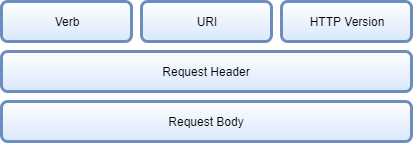
\includegraphics[scale=0.65]{./obrazky-figures/html-request.png}
	\caption{HTTP Request format}
	\label{HTTPRequestFormat}
\end{figure}

\begin{itemize}
  \item \textbf{Verb} indicates the HTTP method like GET, PUT, POST, DELETE,
  etc.
  \item \textbf{URI} is the~Uniform Resource Identifier used~to~identify
  the~resource on~the~server.
  \item \textbf{HTTP Version} is the~version of~HTTP.
  \item \textbf{Request Header} contains the~metadata as~a~collection
  of~\uv{key-value} pairs of~headers and~their values. For~example, client
  (or~browser) type, format supported by~the~client, format of~the~message body,
  cache settings for~the~response, and~a~lot more information.
  \item \textbf{Request Body} is the~actual message content or~resource
  representation.
\end{itemize}

In~the~listing~\ref{GETExample}, we can see an~example of~an~actual GET
request that was created by~the~browser when I tried to~visit the~website
of~Faculty of~Information Technology.

\vspace{2mm}
\begin{lstlisting}[caption=A~sample of~a~simplified GET Request.,
label=GETExample, language=HTML] 
GET / HTTP/1.1
Host: www.fit.vutbr.cz
User-Agent: Mozzila/5.0 (Windows NT 6.3; Win64; x64) ...
Accept: text/html,application/xhtml+xml,application/xml; ...
Accept-Encoding: gzip, deflate
Accept-Language: cs-CZ,cs;
\end{lstlisting}

The~GET command is followed by the URI
and~the~HTTP version. The~request also contains some headers.
The~\uv{User-Agent} header contains information about the~type of~a~client who
made the~request. The~\uv{Accept} headers tells the~server about the~various
representation formats, the encoding and~a~language the~client supports.
The~server, if it supports more than one representation format, can decide
the~format for~a~response at~runtime depending on~the~value
of~the~\uv{Accept} header. Because the~request in~listing~\ref{GETExample} is
a~GET request, it does not contain any message body.

When the~server receives the~request it should respond with a~HTTP Response.
The response has four major parts.

\begin{figure}[!hbt]
	\centering
	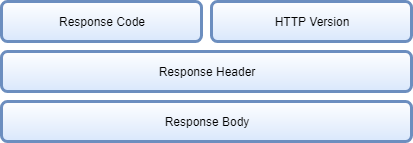
\includegraphics[scale=0.65]{./obrazky-figures/html-response.png}
	\caption{HTTP Response format}
	\label{HTTPResponseFormat}
\end{figure}

\begin{itemize}
  \item \textbf{Response Code} contains the~server status for~the~requested
  resource. This response is generally the~\uv{3-digit} HTTP status code.
  For~example, 404 means resource not found and~200 means
  response is ok.
  \item \textbf{HTTP Version} is the~version of~HTTP.
  \item \textbf{Response Header} contains the~metadata and~settings about
  the~response message as~\uv{key-value} pairs. For example, content length,
  content type, response date, etc.
  \item \textbf{Response Body} contains message content or~resource
  representation if the~request was successful.
\end{itemize}


In~the~listing~\ref{GETExampleResponse}, we can see an~example
of~the~response to~the~GET request to~Faculty
of~Information Technology website we made earlier.

\vspace{2mm}
\begin{lstlisting}[caption=A~sample of~a~simplified response to~a~GET Request.,
label=GETExampleResponse, language=HTML]
HTTP/1.1 200 OK
Date: Sat, 09 Dec 2017 08:36:01 GMT
Server: Apache
Content-Location: index.php.cz
Pragma: no-cache
Keep-Alive: timeout=60, max=100
Connection: Keep-Alive
Transfer-Encoding: chunked
Content-Type: text/html; charset=iso-8859-2
Content-Language: cs
<!DOCTYPE HTML PUBLIC "-//W3C//DTD HTML 4.01//EN">
<html>
<head>
 ...
\end{lstlisting}

The~response code \textit{200 OK} means that everything is ok
and~the~response message body contains a~valid representation of~the~requested resource.
In~this case, the~representation is an~HTML document that is declared
by~\uv{Content-Type} header in~the~response header. The~other attributes
in~the~header are self explanatory.

\subsection{Addressing the Resources}
If we want to~get a~resource from~the~server, we need to~know, how to~address
it. Addressing refers to~locating a~resource or~multiple resources lying
on~the~server. It is analogous to~locate a~postal address of~a~person. A~RESTful
service uses a~directory hierarchy like human readable URIs to~address its
resources. Each resource is identified by~its URI which is of~the~following
format:
\begin{equation*}
<protocol>://<serviceName>/<resourceType>/<resourceID>
\end{equation*}

The~URI should not say anything about the~operation or~action. This enables us
to~call the~same URI with different HTTP verbs to~perform different operations.
Verbs are used to identify the~operation to~be performed on~the~resource.

While designing a~URI some important points should be considered.

\begin{enumerate}
  \item Plural Nouns should be used to~define resources.
  \item Spaces should be avoided. Typically in~URIs it is recommended
  to~use underscore or~hyphen when using a~long resource name.
  \item Lowercase letters are recommended. Although URI is
  \uv{case-insensitive}, it is a~good practice to~keep the~URL in~lower case
  letters only.
  \item Avoid verbs for the~resource names until the~resource is
  actually an~operation or~a~process. 
\end{enumerate}

To~avoid confusion, let us have an~example. Suppose we have a~database
of~users and~we wish to~expose it to~the~Internet through a~service.
We already know that the~resources should be addressed by~the~URI and~the~action
perfomed on~the~resource should be defined by~a~HTTP verb. The~verbs correspond
to~read, create, update, and~delete CRUD\footnote{In~computer programming,
create, read, update, and delete (as~an~acronym CRUD) are the~four basic
functions of~persistent storage.} operations.

\subsubsection{Creating a~user -- POST /users}
To~create new resources, in~this case a~user, the~POST verb is most often
utilized. On~successful creation, returning a~\uv{Location} header with a~link
to~the~newly created resource with the~\textit{201 Created} HTTP status.

The~method is neither safe nor idempotent. It is therefore recommended
for~\uv{non-idempotent} resource requests. Making two identical POST requests
will most likely result in~two resources containing the~same information.

\subsubsection{Retrieving a~user -- GET /users/\{id\}}
The~HTTP GET method is used to~retrieve a~representation of~a~resource, in~this
case a~user with specified id. If the~request is successful, it returns the~user
representation in~XML or~JSON format, like the~one we can see
in~listing~\ref{XMLExample}, respectively \ref{JSONExample},
and~a~HTTP response code of~\textit{200~OK}.

The~GET requests should only be used to~read data and~not change it. Therefore,
when used this way, they are considered safe. That is, they can be called
without risk of~data modification or~corruption. Additionally, the~requests are
idempotent, which means that making multiple identical requests ends up having
the~same result as~a~single request.

\subsubsection{Updating a~user -- PUT /users/\{id\}}
For~update capabilities, the~PUT verb is often most utilized, \uv{PUT-ing}
to~a~known resource, in~our case a~user, with the~request body containing
the~newly updated representation of~the~original resource. On~successful update,
the~server should return \textit{200~OK} or~\textit{204~No~Content} status code
if not returning any content in~the~body. It follows from the~above that a~body in~the~response
is optional -- providing one is not necessary and~only leads to~more
bandwidth consumption.

PUT is not a~safe operation, in~that it modifies state on~the~server, but is
idempotent. In~other words, if we update the~user using the~PUT method and~then
make that same call again, the~resource is still there and~has the~same state 
as~it did with the~first call.

\subsubsection{Deleting a~user -- DELETE /users/\{id\}}
The~DELETE verb is pretty straightforward, it is used to~delete a~resource,
in~our case the~user with specified id. On~successful deletion, the~server
should return HTTP status \textit{204 No Content} with no response body.

\uv{HTTP-spec-wise}, DELETE operations are idempotent. If we delete a~user, it
is removed. Repeatedly calling the~method on~that~user ends up the same --
the~user is gone. There is a~caveat about the~method idempotence, however.
Calling it on~a~resource a~second time will result in~\textit{404~Not~Found}
status code since it was already removed and~therefore is no longer findable. This makes
the~operations in~fact no longer idempotent, however, the~\uv{end-state}
of~the~resource is~the~same.

\subsection{Representation of the Resources}
It is clear that the~focus of~a~RESTful service is on~resources and~how
to~provide access to~them. A~resource can easily be thought of~as~an~object
as~in~OOP\footnote{Object oriented programming (OOP) is a~programming paradigm
based on~the~concept of~\uv{objects}, which may contain data, in~the~form
of~fields; and~code, in~the~form of~procedures, often known as~methods.}. These
resources can be text files, HTML pages, images, or~videos, and~can consist
of~other resources. The~server simply provides access to~resources
and~client accesses and~modifies them. The~architecture does not put
a~restriction on~the~format of~a~resource representation. However,
as~mentioned before, the~most popular representations of~resources are XML
and~JSON.

\vspace{2mm}
\begin{lstlisting}[caption=A XML representation of~a~\textit{user} resource.,
label=XMLExample, language=XML]
<user>
	<id>1</id>
	<firstName>John</firstName>
	<lastName>Doe</lastName>
	<age>42</age>
</user>
\end{lstlisting}

Once a~resource is identified then its representation is to be decided using
a~standard format so that the~server can send the~resource in~the~above
said format and~client can understand the~same format. 

Let us consider an~example of~a~user object. Its XML and~JSON representation can
look like the~one in~the~listing~\ref{XMLExample} and~\ref{JSONExample},
respectively.\\

\begin{lstlisting}[caption=A JSON representation of~a~\textit{user} resource.,
label=JSONExample,language=Java][!hbt]
{
	"id": 1,
	"firstName": "John",
	"lastName": "Doe",
	"age": 42
}
\end{lstlisting}

Despite the~fact that there are no restrictions on~the~format of~a~resource
representation, following some important points should be considered.
For~instance, both the~server and~the~client should be able to understand said
format. Moreover the~format should be able to~represent a~resource completely.

\section{Introduction to~Application Programming Interfaces}
In~computer programming an~application programming interface is the~defined
interface through which interactions happen between an~enterprise and~users
of~its assets. It can become the~primary entry point for~enterprise service,
for~its own website and~applications, as~well as~for~a~partner and~customer
integrations. It is defined through a~contract so~that any application can use
it with relative ease. 

The~API~\cite{RESTfulAPI} approach creates a~loosely coupled architecture that
allows a~component service to~have a~wide range of~future uses, and~is technology agnostic.
The~architecture resolves around providing programmable interfaces to~a~set
of~services to~different applications serving different kinds of~customers. It
assumes that these user groups might change or~evolve over time in~the~way they
utilize the~provided services. The~strategy of~providing APIs leads
to~the~following benefits:

\begin{itemize}
  \item \textbf{Automation}. With APIs, computers rather than people can manage
  the work. Through them, companies can update work flows to~make them quicker
  and~more productive.
  \item \textbf{Integration}. They allow content to~be embedded from any site
  or~application more easily. This guarantees more fluid information delivery
  and~an~integrated user experience.
  \item \textbf{Personalization}. Any user or~company can customize the~content
  and~services that they use the~most.
  \item \textbf{Reduction of costs}. They represent a~cheaper way of~building
  applications by~increasing the~reuse of~services. Providing a~usage or~\uv{analytics-based}
  evolutionary development platform decreases cost of~development and~change
  to~services.
  \item \textbf{Increasing customer loyalty}. The~company that releases
  the~API allows its customers to~access their conferencing services in~new,
  more efficient ways, increasing brand recognition and~customer loyalty.
\end{itemize}

\subsection{When is API RESTful?}
In~the~previous sections we introduced the~term Application Programing
Interface and~explained the~RESTful web services. However, it is necessary
to~point out that not all APIs are considered RESTful. An~API is RESTful only
when it is acting under the~REST constraints at~all times. These constraints
restrict the~ways that the~server may process and~respond to~client requests so
that, by operating within these constraints, the~service gains desirable
\uv{non-functional} properties, such~as~performance, scalability, portability,
and~reliability. These formal constraints are as~follows:

\begin{enumerate}
  \item \textbf{\uv{Client-Server}.} This constraint is based
  on~the~separation of~concerns principle. Separating the~user interface
  concerns from the~data storage concerns improves the~portability of~the~user
  interface across multiple platforms.
  \item \textbf{Stateless.} Communication between client and~server must be
  stateless. This means that each request from~client to~server must contain all
  the~necessary information to~complete the~transaction. The~main advantage
  of~this approach is that the~system is able to~scale better because the~server
  does not have to~store client state between requests.
  \item \textbf{Cacheable.} This constraint ensures that the~clients can cache
  response to~improve performance. \uv{Well-managed} caching partially
  or~completely eliminates some \uv{client-server} interactions, further
  improving scalability and~performance.
  \item \textbf{Uniform Interface.} In~order to~have efficient caching
  in~a~network, components must be able to~communicate via a~uniform interface.
  The~definition of~uniform interface consists of~four other constraints,
  however most of~them can be found implemented in~the~HTTP protocol.
  \item \textbf{Layered System.} In~a~layered system, intermediaries, such
  as~proxies can be placed between client and~server utilising the~web's uniform
  interface. The~main advantage is that intermediaries can then intercept
  \uv{client-server} traffic for~a~specific purposes; for~example caching.
  \item \textbf{Code On Demand.} This is an~optional constraint and~it allows
  clients to~download programs for~\uv{client-side} execution. The~best examples
  for this are compiled components such~as~Java applets or~\uv{client-side}
  scripts such~as~JavaScript.
\end{enumerate}

\subsection{The~Importance of~Testing APIs}
API testing is testing that APIs and~the~integrations they enable work
in~the~most optimal manner. This form of~testing concentrates on~using software
to~make API calls in~order to~receive an~output before observing and~logging
the~system's response. Most importantly, this tests that the~API returns
a~correct response or~output under varying conditions. The~output is typically
as~follows:

\begin{itemize}
  \item A~Pass or~Fail status
  \item Date or~information
  \item A~call to~another API
\end{itemize}

However there also could be no output at~all or~something completely unpredicted
can occur. This makes the~testing a~crucial part of~the~application development
process.

\subsection{The~Frameworks for Testing APIs}
As~APIs are becoming an~integral part of~how software works, and~the~more
the~users rely on~\uv{web-based} systems, the~more crucial is that they are
tested. Therefore it is not a~surprise that there are many frameworks
and~applications that allow to~test the~APIs.

The~simplest is the~cURL~\footnote{The~cURL command line tool can be found
on~\textit{https://curl.haxx.se/}}.
It is a~command line tool for transferring data using various protocols. It
consists of~two products, libcurl and~cURL, where libcurl is a~free \uv{client-side} URL tranfer library and~cURL is
the~actual tool for~getting and~sending files using URL syntax. Together they
allow testing the~APIs using HTTP requests. The~basic use of~cURL involves
simply typing \textit{curl} at~the~command line, followed by~the~URL
of~the~output to~retrieve. As~we can see in~the~listing~\ref{CURLLabel}, writing tests with cURL is not
very intuitive. Therefore, other frameworks and~applications, like the~Postman,
were developed.

\vspace{2mm}
\begin{lstlisting}[caption=An~example of~POST request that creates new user
on~the~server using cURL.,label=CURLLabel,language=XML]
curl -d '{
	"firstName": "John",
	"lastName": "Doe",
	"age": 42
}' -X POST http://localhost:8080/users
\end{lstlisting}

Postman is a~software that allows executing and~managing HTTP requests. It
offers a~\uv{user-friendly} interface with~which is possible to~make
the~requests without the~hassle of~writing code just to~test an~API's
functionality. Using the~user interface, the~developers can simply define
request's address, query parameters, headers, authorization methods and~data,
and~even write simple scripts that are executed before or~after running
the~request. It even supports an~import of~API definitions from the~API
documentation framework Swagger.

However, as~we can see, both of~these applications have a~serious drawback. What
if, a~developer wants to~create test case that would execute first request
and~then took the~response from~the server and~used it as~a~input for~the~second
request? Using cURL this would mean writing additional code that would connect
the~two requests and~in~the~Postman application, this is not possible at~all.
Although Postman offers to~concatenate the~requests into a~collection, it does
not offer to~use one's request output as~other's request input.

\chapter{Technologies and Frameworks}
\label{Technologies}
In~this chapter we will go over the~details of~technologies and~frameworks that
will be used developing the~application. At~first we will introduce the~Swagger
framework. In~next sections the~\uv{front-end} web application framework Angular
along with~the~superset of~EcmaScript~6 -- the~TypeScript language will be
presented. Following the~thesis we will introduce the~web framework
PatternFly and~show its key features for~designing web sites and~web
applications.

\section{Introduction to Swagger Framework}
Swagger is an~open source framework backed by~a~large ecosystem of~tools that
helps developers design, build, document and~test RESTful web services. It
allows to~describe the~structure of~the~APIs so that machines can read them.
By~reading the~API's structure, the~framework can automatically build an~API
documentation. It does this by~asking the~API to~return a~YAML or~JSON that
contains a~detailed description of~the~entire API. The~file is essentially
a~resource listing of~the~API which adheres to~OpenAPI
Specification\footnote{The~OpenAPI Specification is a~specification
for~\uv{machine-readable} interface files for~describing, producing, consuming,
and~visualizing RESTful web services.}. Developers can write the~specification
for~the~API manually or~have it generated automatically from~annotations
in~the~source code.

\subsection{Generating the API Documentation}
To~clarify how the~Swagger works, let us consider an~example. In~the~example we
are going to~use Swagger on~top of~Spring Framework, however keep in~mind that
the~Swagger is a~specification, and supports a~wide range of~frameworks. Swagger
supports various annotation like the~\textit{@Api} for~instance, that allows
developers to~specify details of~the~documentation.

\vspace{2mm}
\begin{lstlisting}[caption=An~example of~Swagger's internal annotation that can
be used to~generate documentation., language=Java,
label=SwaggerAnnotation]
@RestController
@RequestMapping("/users")
@Api(value = "users", description = "Users endpoints")
public class UsersController { ... }
\end{lstlisting}

The~alternative way is to~let Swagger figure out the~documentation by~itself
based on~the~annotations from~Spring Framework. Under the~hood, it scans
the~Spring controllers on~\uv{start-up} and~registers a~documentation controller that exposes the~operations
the~controller allows. The~documentation follows the~specification -- any client
that understands the~specification can use the~API. The~important thing is that
the~documentation is based on~the~code itself, therefore any change to~the~code
is reflected on~the~documentation. There is no need to~maintain an~external
document. 

\vspace{2mm}
\begin{lstlisting}[caption=An~example of~Spring MVC controller that can be used
by~Swagger to~generate API documentation., language=Java,
label=SpringController]
@RestController
@RequestMapping("/users")
public class UsersController {
	
	@Autowired
	private UserService userService;
	
	@PostMapping
	@ResponseStatus(HttpStatus.CREATED)
	public User createUser(@RequestBody UserDto userDto) {
		return userService.createUser(userDto);
	}
	
	@GetMapping
	@ResponseStatus(HttpStatus.OK)
	public List<User> findAllUsers() {
		return userService.findAllService();
	}
	
	@DeleteMapping
	@ResponseStatus(HttpStatus.NO_CONTENT)
	@RequestMapping(value = "/users/{userId}"
	public void deleteUserById(@PathVariable Long userId) {
		userService.deleteUserById(userId);
	}
	
}
\end{lstlisting}

The~documentation then consists of~2 parts, as~shown
in~the~listing~\ref{SwaggerJSON}, the~operations and~the~models. We can
see that a~client can send a~GET request on~the~\textit{/users} endpoint
to~select the~users. This is an~example of~an~operation. Following the~code, we can see that the~operation returns
a~list of~users of~which a~client can learn more in~the~models section.

However, the~main advantage of~the~framework is that it exposes
the~endpoints from~the~documentation controller and~makes them accessible
on~the~\textit{/api-docs} URL. Therefore we can build the~application upon it
plus any developer who uses the~framework, will be able to~use the~result
of~the~thesis for~testing his own application.
\pagebreak

\begin{lstlisting}[caption=An~example of~documentation in~JSON format
generated by~the~Swagger framework from~code
in~the~listing~\ref{SpringController}., language=XML, label=SwaggerJSON]
{
	"apiVersion": "1.0",
	"swaggerVersion": "1.0",
	"basePath": "http://localhost:8080",
	"resourcePath": "/users",
	"apis": [
		{
			"path": "/users",
			"description": "users",
			"operations": [
				{
					"httpMethod": "GET",
					"summary": "findAllUsers",
					"notes": "",
					"deprecated": "false",
					"responseClass": "List[User]", 
				},
				
				... 
			]
		}
	],
	"models": [
		"User": {
			"properties": {
				"id": {
					"type": "long"
				},
				"firstname": {
					"type": "string"
				},
				"lastname": {
					"type": "string"
				}
			}
		}
		
		...	
	]
}
\end{lstlisting}

\section{What is Angular?}
Angular~\cite{Angular} is an~open source TypeScript framework used to~build web
applications in~HTML and~TypeScript. It makes it easy to~build application as~it
combines declarative templates, dependency injection, end to~end tooling, and~integrated best practices to~solve development challenges.

\subsection{Beginning as AngularJS}
Angular originally started as~AngularJS when it was developed in~2009 by~M.
Hevery~\cite{HeveryAngularJS} as~the~software behind an~online JSON storage
service, that would have been priced by~the~megabyte, for~\uv{easy-to-make}
applications for~the~enterprise. However, the~business idea was abandoned
and~AngularJS was released as~an~open source library in~October 2010.

The~framework was used to~overcome obstacles encountered while working
with~Single Page applications\footnote{A~single page application (SPA) is a~web
application or~web site that interacts with the~user by~dynamically rewriting
the~current page rather than loading entire new pages from a~server.}.
However, because some of~the~core assumptions in~AngularJS needed to~be changed,
in~September 2016 saw the~light of~the~day a~complete rewrite of~AngularJS.
Originally, the~rewrite was called \uv{Angular 2} by~the~team that built it, but
this led to~confusion among developers. To~clarify, the~team announced that
separate terms should be used for~each framework with \uv{AngularJS} referring
to~the~1.X versions and~\uv{Angular} without the~\uv{JS} referring to~version~2
and~up.

As~the~new version of~the~framework was developed, some new concepts appeared.
In~addition to~better \uv{event-handling} capabilities, powerful templates,
and~better support for~mobile devices, Angular introduced several new features.

\begin{enumerate}
  \item \textbf{Components} -- The~earlier version of~Angular had~a~focus
  of~Controllers, but now has changed the~focus to~having components over
  controllers. They help to~build applications into many modules, which
  helps in~better maintaining the~application over~a~period of~time.
  \item \textbf{TypeScript} -- The~newer version of~Angular is based
  on~TypeScript. It is a~superset of~JavaScript maintained by~Microsoft. We will
  learn more about TypeScript later in~section~\ref{TypeScript}.
  \item \textbf{Services} -- are a~set of~code that can be shared by~different
  components of~an~application. So~for~example if we had a~data component that
  picked data from~a~database, we could have it as~a~shared service that could
  be used across multiple applications.
\end{enumerate}

\subsection{Angular's Core Concepts}
As~mentioned in~previous section, Angular introduces the~two core concepts --
components and~services, respectively the~dependency injection.

An~Angular application will always have a~root component that contains all other
components. In~other words, an~application will always have a~component tree,
in~which components are~a~logical piece of~code that consists of~following.

\begin{enumerate}
  \item \textbf{Template} that is used to~render the~view for~the~applications.
  It contains the~HTML that needs to~be~rendered as~well as~the~bindings
  and~directives.
  \item \textbf{Class} is like a~class defined in~any~language such~as~C except
  it is defined in~TypeScript. Classes contains properties, methods,
  and~the~code which is used to~support the~view.
  \item \textbf{Metadata} contains an~extra data defined for~the~Angular class.
  They are defined with~a~decorator.
\end{enumerate}

\pagebreak
\begin{lstlisting}[caption=An Angular class with the~\textit{@Component}
decorator and~a~template., label=AngularComponent, language=HTML]
@Component ({
	selector: 'my-app-hello-world',
	template: `
		<div>
			<h1>{{title}}</h1>
		</div>
	`,
})
export class HelloWorldComponent {
	title: string = 'Hello World!';
}
\end{lstlisting}

In~the~listing~\ref{AngularComponent} we can see an~example of~the~completed
code with class, template and~metadata. We are defining a~class in~TypeScript
called \textit{HelloWorldComponent} that contains only one property --
\textit{title}. Using the~\textit{@Component} decorator we define a~component
and~inside the~decorator we can then define the~HTML template, which is the~view
that needs to~be rendered in~the~application.

The~second cornerstone of~an~Angular application is dependency injection.
The~idea behind it is pretty simple. If we have a~component that depends
on~a~service, we do not create the~service ourselves. Instead we request one
in~the~constructor and~the~framework will provide us one. By~doing so, we can
depend on~interfaces rather than concrete types. This approach leads to~more
decoupled code, which enables testability and~other great things.

\begin{figure}[!hbt]
	\centering
	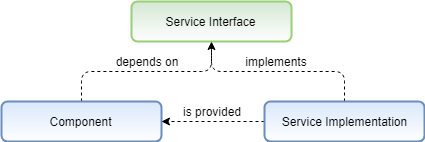
\includegraphics[scale=0.65]{./obrazky-figures/DI.png}
	\caption{Angular's way of~injecting and~instantiating services
	in~the~components.}
	\label{DependencyInjection}
\end{figure}

To~clarify, let us consider an~example. In~the~listing~\ref{AngularService} we
defined a~simplified service that has a~method that returns an~array of~users.
If~we create a~component and~specify an~argument of~type~\textit{UserService}
in~that component, Angular will automatically instantiate and~inject
the~\textit{UserService} into the~component.

As~we can see the~Angular's dependency injection
module is flexible, and~easy to~use because the~objects can be injected only via
constructors. In~addition, the~injectors form a~hierarchy, and~the~injectable
object does not have to~be an~\uv{application-level} singleton as~it might
by~default in~Spring Framework\footnote{The~Spring Framework is an~application
framework and~inversion of~control container for~the~Java platform.}
for~example.

\pagebreak
\begin{lstlisting}[caption=An example of simple dependency injection in
Angular., label=AngularService,language=HTML]
export class UserService {
	users: User[] = [];
	
	findUsers(): User[] {
		// Here should be the code used to retrieve the users
		return users;
	}
}

	

@Component {
	...
}
export class UsersComponent {
	users: User[] = [];
	
	constructor(userService: UserService) {
		this.users = userService.findUsers();
	}
}
\end{lstlisting}

\section{Introducing~TypeScript}
\label{TypeScript}
In~September 1995 was first intoduced JavaScript as~a~language for~the~client
side. It was used to~make webpages interactive and~to~provide online programs,
including video games. However, as~JavaScript code grows, it tends to~get
messier, making it difficult to~maintain and~reuse the~code. Moreover, its
failure to~embrace the~features of~Object Orientation, strong type checking
and~\uv{compile-error} checks prevent JavaScript from succeeding
at~the~enterprise level as~a~\uv{full-fledged} server side technology.
TypeScript was presented to~bridge this gap. Its main goals were to~provide
an~optional type system and~planned features from future JavaScript editions
to~current JavaScript engines.

\subsection{Why Add Types to JavaScript}
Types have proven ability to~enhance code quality and~understandability.
Increasing the~agility when doing refactoring and~being one of~the~best forms
of~documentation a~developer can have. However, types have a~way of~being
unnecessarily ceremonious. Therefore TypeScript is very particular about keeping
the~barrier to~entry as~low as~possible, only providing compile type safety
for~the~JavaScript code. The~great thing is that the~types are completely
optional. 

TypeScript provides data types as~a~part of~its optional type system. As~a~super
type of~all types, the~\textit{any} data type is used. It denotes a~dynamic type
and~using it is equivalent to~opting out of~type checking for~a~variable. That
suggests that the~variable may be declared with no type which means that
the~type of~the~varible will be inferred by~the~TypeScript Language Service.
All~other \uv{built-in} types and~\uv{user-defined} types inherit from
the~\textit{any} type.

\pagebreak
\begin{lstlisting}[caption=An~example of~TypeScript's type inference. The~type
of~the~variable is inferred by~the~TypeScript Language Service based on~its
value.,
label=TypeScriptInference,language=HTML]
var foo = 42;
foo = 'Hello World!';

// The previous line will throw an error: 
// 	   cannot assign `string` to `number`
\end{lstlisting}

Important to~mention is that the~\uv{built-in} types \textit{undefined}
and~\textit{null} may look similar but are not the~same. A~variable initialized
with~\textit{undefined} means that the~variable has no value or~object assigned
to~it, while \textit{null} means that the~variable has been set to~an~object
whose value is undefined.

\begin{figure}[!hbt]
	\centering
	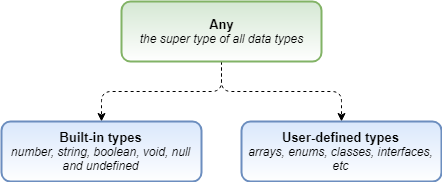
\includegraphics[scale=0.65]{./obrazky-figures/typescript-types.png}
	\caption{Data type classification in TypeScript.}
	\label{TypeScriptDataTypes}
\end{figure}

The~main advantage is however that the~JavaScript code files with the~\uv{.js}
suffix can be renamed to~a~files with \uv{.ts} suffix and~TypeScript will give
back a~valid equivalent to~the~original JavaScript file. That is because
TypeScript is intentionally and~strictly a~superset of~JavaScript with~optional type checking.

\subsection{Future JavaScript}
The~second goal of~TypeScript was to~provide planned features from future
JavaScript editions. Nowadays, it provides a~number of~features that are planned
in~EcmaScript 6\footnote{The~EcmaScript specification is a~standardized
specification of~a~scripting language.} for~current JavaScript engines.
For~instance, the~language features modules and~\uv{class-based} orientation
as~well as~features like generics and~type annotations that are not a~part
of~the~specification.

In~conclusion, even thought we could use JavaScript with Angular, TypeScript
feels like a~superior choice, not only because it is strongly typed and~supports
object oriented programming, but because of~the~TypeScript's transpiler which
provides the~\uv{error-checking} feature. Unlike JavaScript,
the~TypeScript is not an~interpreted language and~will compile the~code
and~generate compile errors if it finds some sort of~syntax errors. Thus
helps to~highlight the~errors before the~script is run hence, saving time trying
to~find the~bugs in~the~code.

\section{Styling with PatternFly}
The~success of~an~application depends on~a~\uv{well-designed} user interface.
The~good or~bad design can influence the~perceived usability of~an~application,
and~if the~application design is not done well, the~whole application can be
perceived as~bad. The~PatternFly framework was developed specifically to~address
this issue.

One of~the~main things that sets the~framework apart from other libraries is
the~focus on~design for IT enterprise applications. It recognizes the~importance
for~a~user to~be able to~migrate seamlessly from one product to~another without
having to~relearn the~UI. Behavioral consistency leads to~better usability
because users are familiar with the~interactions. Visual consistency establishes
a~look and~feel that users recognize and~allows to~unify disparate projects,
make them look great and~make them look like they belong in~the~same portfolio.

PatternFly is an~open source project that is based
on~Bootstrap~\cite{Bootstrap}, a~\uv{mobile-first} frontend framework
for~creating web sites and~applications. It is developed using
Less, a~cascading style sheet
\uv{pre-processor} that extends the~CSS language and~adds features that allow
variables, mixins, functions, and~many other techniques that allow developers
create code that is more maintainable, themeable and extendible. This allows
the~developer to~add any required \uv{app-specific} CSS directly into one CSS
file, which is more performant, and~make any necessary adjustments to~PatternFly
via variable overrides.

The~framework consists of~a~series of~Less stylesheets that implement
various components of~the~toolkit. These stylesheets are generally compiled into
a~bundle and~included in~web pages, but individual components can be included
or~removed. Moreover it provides a~number of~variables that control things such
as~color and padding of~various components. Each component consists
of~a~HTML structure and~CSS declarations, and in~some cases
accompanying JavaScript code.

\subsection{Using the Components}
PatternFly comes with various design templates for~typography, tables, forms,
buttons, navigation, and~other interface components that can be used building
the~application --~saving lots of~time and~efforts in~the~process. These
templates are made available as~\uv{well-factored} CSS classes that
the~developers can apply to~the~HTML to~achieve different effects.
By~using semantic class names like \textit{.alert} and~\textit{.alert-success},
these components are easily reusable and~extensible. Although the~framework uses
descriptive class names that have meaning, it is not specific about
implementation details. Therefore all classes can be overriden with custom
CSS style and still the~meaning of~the~class will remain
the~same.

\vspace{2mm}
\begin{lstlisting}[caption=An~example of~\textit{alert} implemented using
the~PatternFly framework.,language=HTML,label=PatternFlyAlert]
<div class="container">
	<div class="alert alert-success">
		<span class="pficon pficon-ok"></span>
		<strong>Hello World!</strong>
		<span>This is an example of an alert in PatternFly</span>
	</div>
</div>
\end{lstlisting}

To~clarify, the~following code snippet in~the~listing~\ref{PatternFlyAlert} will
generate an \textit{alert} component with the~\uv{Hello World!} text. Using
the~semantic class names, the~code is easily styled allowing the~developer to
spend more time on~application specific features and~functions rather than
application designs.

\begin{figure}[!hbt]
	\centering
	
\includegraphics[scale=0.7]{./obrazky-figures/patternfly-components.png}
	\caption{The~result of~styling the~components with~PatternFly using the~code
	in~listing~\ref{PatternFlyAlert}}
	\label{PatternFlyComponents}
\end{figure}

\subsection{Working with the Grid}
In~the~beginning we mentioned that the~PatternFly, respectively its predecessor
Bootstrap was developed with~a~\uv{mobile-first} design philosophy, which
resulted in~a~framework that is responsive by~design. The~end result is that it
easily and~efficiently scales with~a~single code base, from~phones, through
tablets, to~desktops. This responsiveness is achieved using a~fluid grid system
that can be applied to~appropriately scale~up to~12~columns according
to~the~size of~the~device or~viewport. Grids provide structure to~the~layout,
defining the~horizontal and~vertical guidelines for~arranging content
and~enforcing margins.

To~use the~grid system, a~few rules need to~be followed. Grid column elements
are placed inside row elements, which create horizontal groups of~columns. It is
possible to~have as~many rows as~we want on~the~page, but columns must be
immediate children of~rows. In~a~full row, the~column widths will be any
combination that adds up~to~12, but it is not mandatory to~use all available
columns.

\vspace{2mm}
\begin{lstlisting}[caption=An~example of~the~grid system
in~PatternFly.,label=PatternFlyGrid,language=HTML]
<div class="container">
	<div class="row">
		<div class="col-md-6">First column</div>
		<div class="col-md-6">Second column</div>
	</div>
	<div class="row">
		<div class="col-md-3">First column</div>
		<div class="col-md-3">Second column</div>
		<div class="col-md-3">Third column</div>
		<div class="col-md-3">Fourth column</div>
	</div>
</div>
\end{lstlisting}
  
The~rows needs to~be places in~a~\uv{fixed-width} layout wrapper that has
a~\textit{.container} class and~a~width of~1170px or~in~\uv{full-width} layout
wrapper, which has~a~\textit{.container-fluid} class, and~which enables
the~responsive behavior in~that row. The~grid system is based on~four tiers
of~classes -- \textit{xs} for~phones, \textit{sm} for~tablets, \textit{md}
for~desktops and~\textit{lg} for~larger desktops. These define the~sizes
at~which the~columns will collapse or~spread horizontally. To~clarify, let us
consider an~example with~two rows, one with~two columns, and~one with~four, such
as~in~listing~\ref{PatternFlyGrid}.


% ==============================================================================


\chapter{Application Design}
\label{Design}
% TODO
TODO -- introduction to designs

\section{Application's Requirements}
% TODO 
TODO -- requirements for the resulting application

\section{Wireframes}
% TODO
TODO -- app's wireframes


% ===============================================================================


\chapter{Conclusion}
% TODO
TODO - conclusion

%https://blog.readme.io/what-is-swagger-and-why-it-matters/

%================================================================================
